\section{Introduction}
\label{sec:introduction}
Embedding-model upgrades create an index-maintenance problem: destination-model queries must remain effective while legacy document vectors are replaced gradually. A staged migration learns from paired embeddings, maps the remaining documents, and replaces these proxies as true destination vectors become available. We seek strong intermediate retrieval with limited destination-document exposure.

The intermediate index must rank true destination embeddings and mapped proxies together. A mapper that works well on a proxy-only gallery can change behavior after true vectors are inserted. Cosine retrieval also depends on direction, whereas coordinate regression spends capacity on radial errors that disappear after normalization. This motivates a directional document adapter that preserves compact inference and searches with the native destination query.

Document conversion and query adaptation bridge embedding spaces~\cite{embeddingconverter,driftadapter}; orthogonal alignment, local alignment and neural regression offer different flexibility~\cite{la2m,simplelinear}. We correct the prediction error that changes direction while retaining one affine document map.

\method\ applies two tangent corrections to centered rectangular Procrustes. Each projects destination error onto the tangent plane at the predicted direction, rescales it to the raw prediction, and fits an affine ridge update. Both updates collapse into one affine map followed by normalization. Native destination queries search true and proxy vectors together; each encoded document replaces its proxy under the same identifier (Fig.~\ref{fig:mechanism}).

The results identify a strong quality--exposure trade-off. On four development collections, the fixed 1,024-pair adapter leads all five baseline configurations in macro \ndcg\ across two migrations and three budgets, gaining 0.0243 over Procrustes. The second correction adds 0.0069 without adding an inference stage. On the prospective TREC-COVID collection, E5 gains over Converter and ridge persist at every budget. Across all five collections, E5 ARC2 at 25\% coverage also exceeds these two alternatives at 75\% in a descriptive comparison. Matched all-paid fitting strengthens MiniLM adaptation by another 0.0596 nDCG at the same paid-document budget.

\noindent\begin{minipage}{\linewidth}
Our contributions are:
\begin{itemize}
  \item \textbf{Directional refinement with affine inference.} Two tangent-residual ridge updates target prediction direction and improve measured development retrieval while retaining one compact document map and native destination queries.
  \item \textbf{Strong quality at matched fitting exposure.} Across two migrations and three paid-document budgets, the four-collection development macro favors \method\ over all five evaluated alternatives. Ablations test the second update and directional targeting under matched initialization; all-paid fitting tests larger supervision.
  \item \textbf{Useful quality at lower document exposure.} A held-collection evaluation confirms E5 gains over Converter and affine ridge at each tested budget. The descriptive 25\%-versus-75\% comparison exposes a useful migration operating point, while mixed-gallery diagnostics explain why adapter choice must be evaluated after native-vector insertion.
\end{itemize}
\end{minipage}

\begin{figure}[t]
\centering
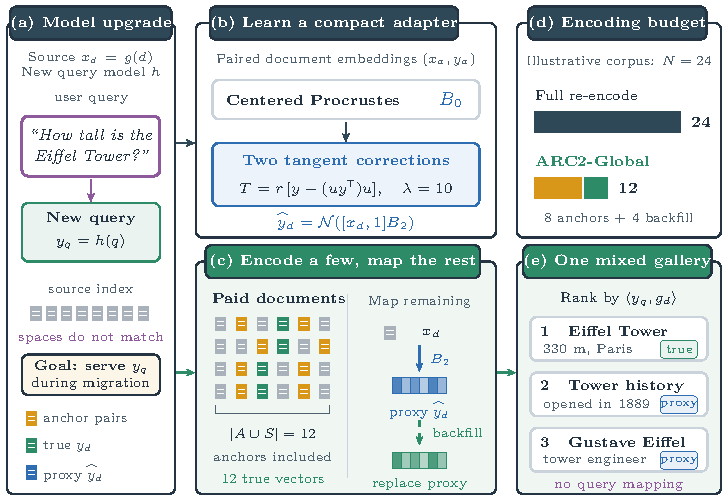
\includegraphics[width=\linewidth]{mechanism.pdf}
\caption{A worked \method\ migration. Paired document vectors train centered Procrustes and two tangent corrections, yielding one affine adapter. Unencoded documents remain searchable through proxies; backfill replaces them with native vectors in the same gallery. The 24-document corpus, eight anchors, four additional encodings and displayed hits are illustrative, not measured retrieval results.}
\label{fig:mechanism}
\end{figure}
